\documentclass[12pt,a4paper,article,english,firamath]{nsi}
\pagestyle{empty}
\setfontfamily{\brettley}{Cursive standard}[Scale=1.5]
\begin{document}
\titre{Find your figure}
\classe{Euro 1\ere}
\maketitle

\subsection*{Description 6}
{\brettley 

Draw a segment line, its midpoint, and a circle whose center is the midpoint and passing through the endpoints of the segment line. Draw a line perpendicular to it passing by its midpoint and then, passing by the two intersections with the circle, draw two lines parallel to this same segment. Finally, choose an endpoint of the segment line and draw perpendicular line passing through it.}\\[1em]

\begin{tikzpicture}
    \draw[lightgray](0,0)--(\linewidth,0);
\end{tikzpicture}


\subsection*{Figure 8}
\begin{center}
    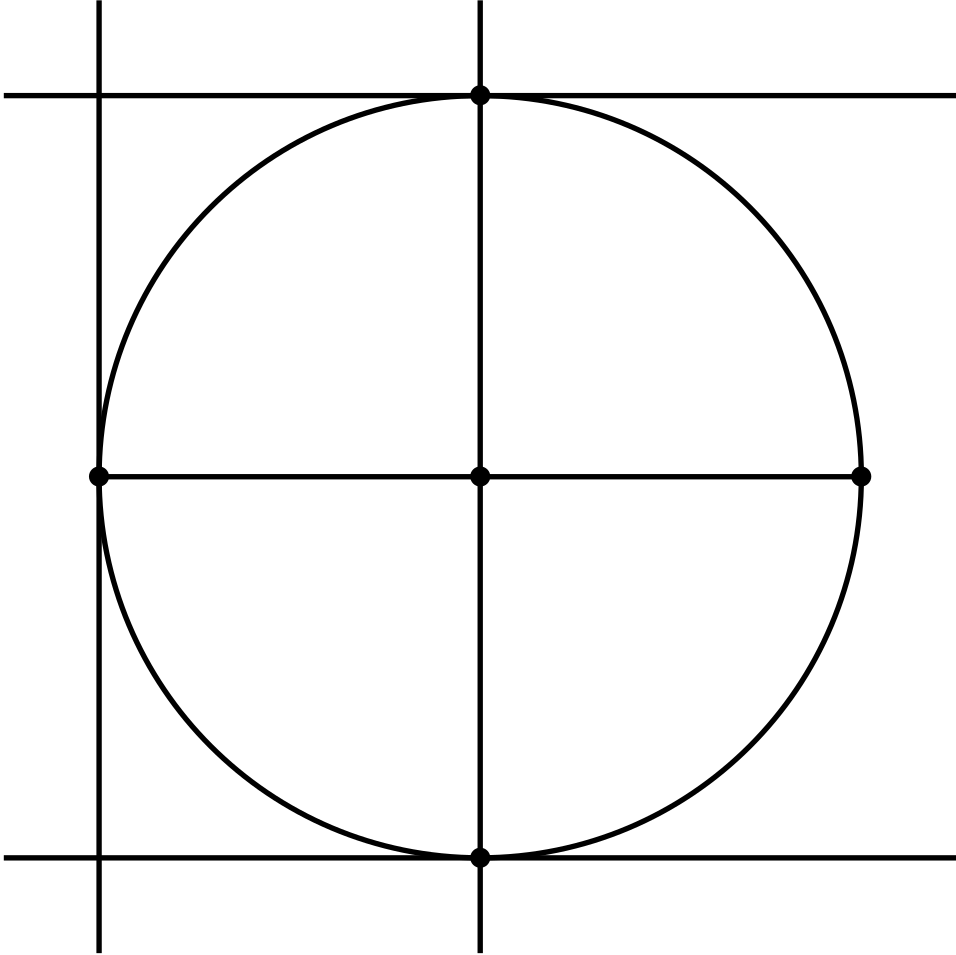
\includegraphics[height=12cm]{img/fig06.png}
\end{center}
\end{document}